\documentclass[border=10pt]{standalone}

\usepackage{tikz}
\usepackage{tikzsymbols}
\usetikzlibrary{calc,patterns,shapes.geometric}

\def\centerarc[#1](#2)(#3:#4:#5){\draw[#1] ($(#2)+({#5*cos(#3)},{#5*sin(#3)})$) arc (#3:#4:#5);}

\begin{document}
	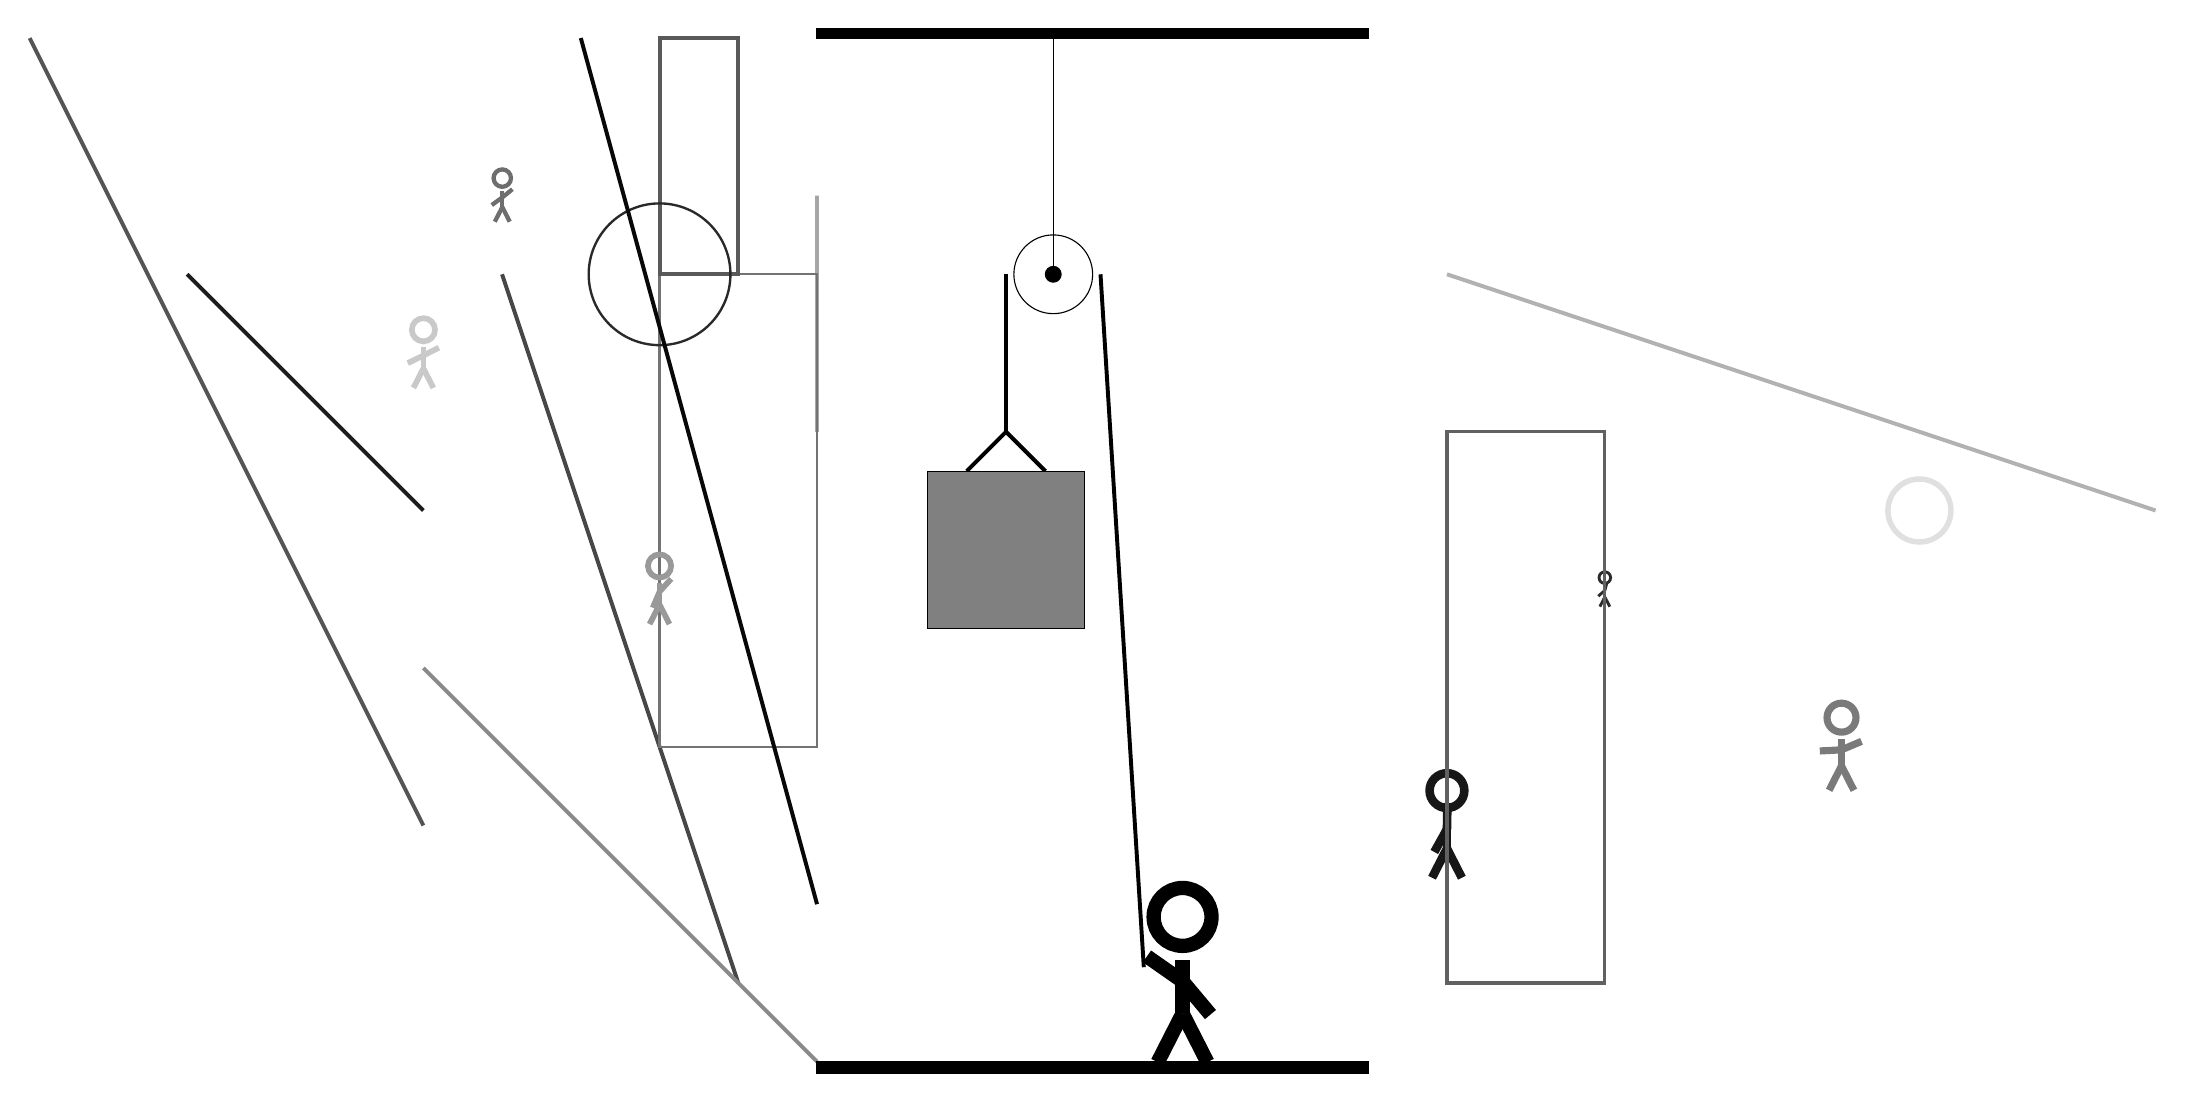
\begin{tikzpicture}
		%%%%% START %%%%%
		
		\draw[fill=black] (-2, 10) rectangle (5, 10.125);
		
		\draw (1, 7) circle (0.5);
		\draw[fill=black] (1, 7) circle (0.1);
		\draw (1, 10) -- (1, 7);
		
		\draw[line width=0.5mm, color=black!35] (-2, 5) rectangle (-2, 8);
		
		\draw [line width=0.7mm, color=black!12](12, 4) circle (0.4);
		\draw[line width=0.5mm, color=black!72](-6, 7) -- (-3, -2);
		\draw[line width=0.5mm, color=black!46](-7, 2) -- (-2, -3);
		\node[line width=0.5mm, color=black!57] at (-6, 8) {\Strichmaxerl[3][36][39]};
		\draw[line width=0.3mm, color=black!55] (-2, 7) rectangle (-4, 1);
		
		\draw[line width=0.5mm, color=black!65] (-4, 10) rectangle (-3, 7);
		\draw[line width=0.5mm, color=black!89](-7, 4) -- (-10, 7);
		\node[line width=0.5mm, color=black!21] at (-7, 6) {\Strichmaxerl[4][26][27]};
		\node[line width=0.7mm, color=black!40] at (-4, 3) {\Strichmaxerl[4][67][48]};
		
		\draw [line width=0.3mm, color=black!84](-4, 7) circle (0.9);
		
		\draw[line width=0.5mm, color=black!67](-7, 0) -- (-12, 10);
		\draw[line width=0.5mm, color=black!30](6, 7) -- (15, 4);
		
		\node[line width=0.5mm, color=black!52] at (11, 1) {\Strichmaxerl[5][3][23]};
		\node[line width=0.6mm, color=black!91] at (6, 0) {\Strichmaxerl[6][61][89]};
		\node[line width=0.6mm, color=black!83] at (8, 3) {\Strichmaxerl[2][41][75]};
		
		\draw[line width=0.5mm, color=black!97](-5, 10) -- (-2, -1);
		
		\draw[line width=0.4mm, color=black!62] (6, 5) rectangle (8, -2);
		
		\draw[line width=0.5mm] (-0.1, 4.5) -- (0.4, 5.0) -- (0.9, 4.5);
		\draw[fill=black!50] (-0.6, 4.5) rectangle (1.4, 2.5);
		
		\draw[line width=0.5mm] (0.4, 7) -- (0.4, 5.0);
		\centerarc[line width=0.5mm](1, 7)(0:180:0.6);
		\draw[line width=0.5mm](1.6, 7) -- (2.15, -1.8);
		
		\node at (2.6, -1.9) {\Strichmaxerl[10][-35][-50]};
		
		\draw[fill=black] (-2, -3) rectangle (5, -3.15);
		
		%%%%% END %%%%%
	\end{tikzpicture}
\end{document}